\chapter{Methoden}
\label{sec:Chapter2}


\section{Bloom Filter}
\label{sec:Sec1.2}


Alle in diesem Praktikum vorgestellten Algorithmen basieren auf Bloomfiltern.
Hierbei handelt es sich um eine Technik, welche dazu dient festzustellen, ob bestimmte Daten in einem Datensatz enthalten sind oder nicht.
Bloomfilter setzen sich zusammen  aus einem mit Nullen vorinitialisiertem $m$ Bit langen Array und einer Anzahl von k Hashfunktionen, welche auf die Positionen des Arrays abbilden.

Zur Initialisierung werden auf jedes Element des Datensatzes alle k Hashfunktionen angewendet.
Die zur Ausgabe der Hashfunktionen korrespondierenden Bits im Array werden darauf hin auf Eins gesetzt.

Soll für ein Datenelement geprüft werden, ob dieses Teil des Datensatzes ist, werden  alle Hashfunktionen auf dieses angewendet.\\
Nur wenn alle Positionen im Array an den korrespondierenden Punkten der Ausgabe dem Wert Eins entsprechen wird angenommen das sich das Element im Datensatz befindet.

Diese Überprüfung ist jedoch nicht resistent gegenüber Falsch Positiven Ergebnissen, da diese Positionen auch durch mehrere Funktionen beschrieben werden kann
\begin{figure}[htbp] 
	\centering
	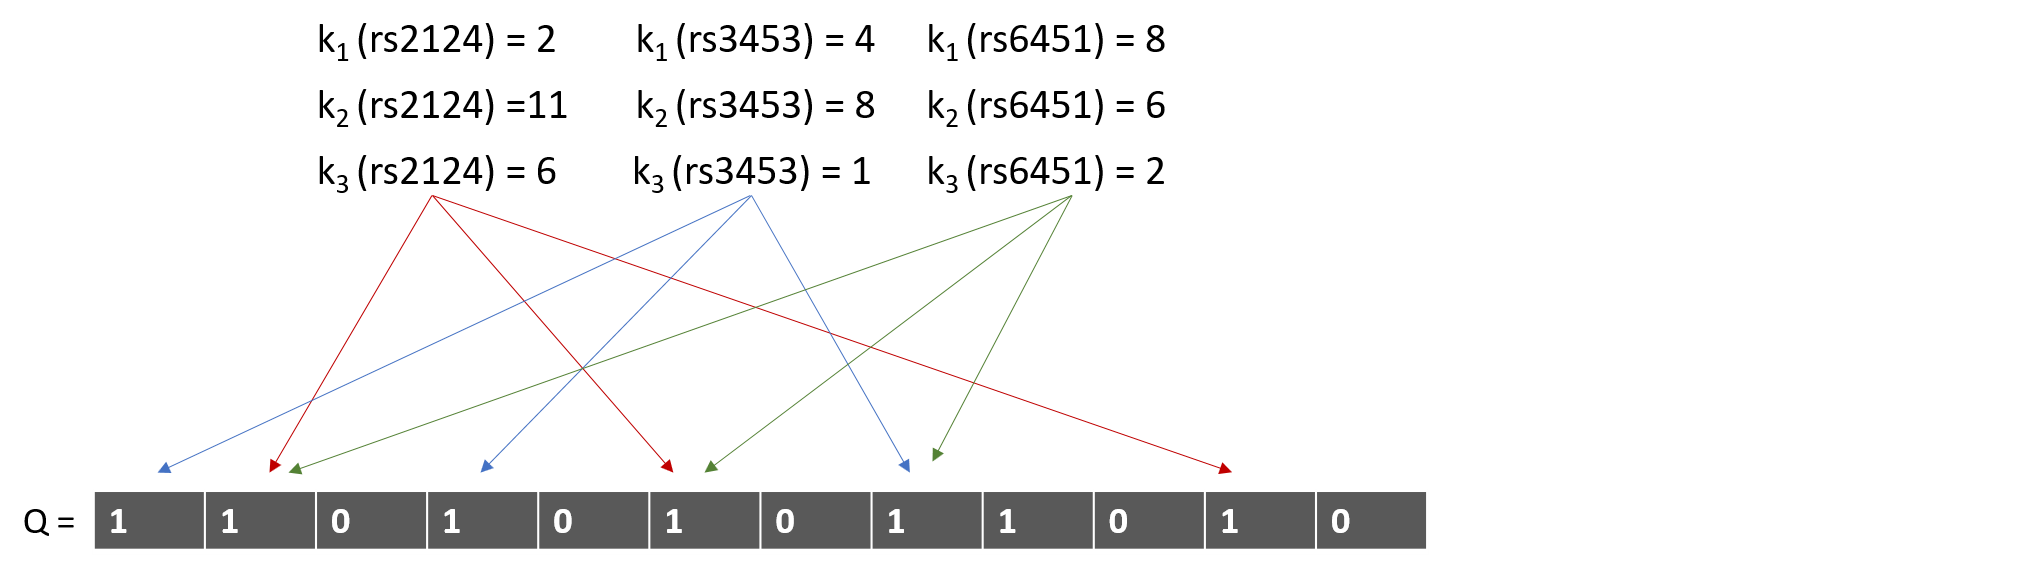
\includegraphics[width=1.2\textwidth]{Graphics/bloomfilter2.png}
	\caption{Initialisierung eines Bloomfilter Q vom 3 SNPs, k=3 Hashfunktionen und einem m=12 Bit langem Array }
	\label{fig:Bild2}
\end{figure}

\section{Kryptosysteme}
\label{sec:Sec1.3}

\subsection{Homomorphie}
Homomorphie bezeichnet eine Eigenschaft von Kryptosystemen. 
Ein Kryptosystem ist genau dann homomorph gegenüber einer mathematischen Operation, wenn Berechnungen im Ciphertext mit dieser Operation denen im KLartext entsprechen.

\subsection{Elgamal}
\label{sec:Sec1.3.1}


Bei dem Kryptosystem Elgamal handelt es sich um ein im Jahr 1985 vom Kryptologen Taher Elgamal entwickeltes Public-Key-Verschlüsselungsverfahren. Elgamal ist eine Erweiterung des Diffie-Hellmann
Schlüsselaustausches.

\textbf{Verfahren}\\

Zunächst wählt der Client eine endliche zyklische Gruppe Z der Ordnung q mit einem Generator g.
\begin{itemize}	
	\item Secrect key: Der Client wählt eine zufällige Zahl $a<q$ mit dem $GGT(a,q) = 1$. Dies ist der Secret key
	\item Public Key: Der public key ist dann $P = g\textsuperscript{a} $	
\end{itemize}

Sei $m \in Z\textsubscript{q}$ die zu versendende Nachricht. Dann wählt der Server eine zufällige Zahl $r<q$ mit dem $GGT(r,q) = 1$. Nun berechnet sich $c\textsubscript{1} = g\textsuperscript{r}$ sowie $c\textsubscript{2} =P \textsuperscript{r} *m$. Der Ciphertext besteht so aus $C = (c\textsubscript{1},c\textsubscript{2})$.

Zur Entschlüsselung wird $\Sigma = c_{1}^{-q} * c_{2} brechnet.$

\textbf{Homomorphie}\\
Elgamal ist homomorph gegenüber der Multiplikation
$$ E(m \textsubscript{1} * m \textsubscript{2}) = (E(m \textsubscript{1}) * E(m \textsubscript{2}))$$

\textbf{Sicherheit}\\
Elgamal ist IND-CPA sicher, falls das



Dann gibt es einen Algorithmus, der in polyn. Zeit DH-Schlussel gab von zufälligen Gruppenelementen unterscheidet.
Widerspruch:
Nach Annahme gibt es keinen effizienten
Algorithmus zum Entscheiden von DH-Schlusselngab.
Daher kann es auch keinen polynomiellen Angreifer A geben.



\subsection{Pailier}

\label{sec:Sec1.3.2}

\textbf{Verfahren}\\
\\
\textit{Schlüsselerzeugung:}\\
Das Schlüsselpaar wird folgendermaßen generiert:
Der Client wählt zwei Primzahlen p,q , mit ggt(pq, (p-1)(q-1))= 0. Des weiteren wird der Generator g so gewählt, sodass $ g \in (\mathbb{Z}/ n^{2} \mathbb{Z}) $ und$ n $ die Ordnung von g teilt.
Das Schlüsselpaar wird dann folgendermaßen gebildet.
\begin{itemize}	
	\item Secrect key: $ \lambda = kgV(p-1, q-1) $
	\item Public Key: $(n,g)$	
\end{itemize}

\textit{Verschlüsselung:}\\
Zur Verschlüsselung einer Nachricht $ m \in \mathbb{Z} $ wählt der Client zunächst eine Zufalls Zahl $ r $ wobei $ 0 \leq r \leq n $\\
Dann berechnet sich der Ciphertext $ c = g^{m}*r^{n} \mod\ n^{2} $\\
\textit{Entschlüsselung:}\\
Der Plaintext kann folgendermaßen berechnet werden: $ m = L(c^{\lambda} \mod n^{2}) * \mu mod n $\\
\\
\textbf{Homomorphie:}\\
Paillier ist homomorph gegenüber der Addition.

$$ E(m \textsubscript{1} + m \textsubscript{2}) = (E(m \textsubscript{1}) + E(m \textsubscript{2}))$$

\textbf{Sicherheit}\\
 

\subsection{Goldwasser-micali}
\label{sec:Sec1.3.3}

\textbf{Verfahren:}\\

\textit{Schlüsselerzeugung:}\\
Zunächst generiert der Client zwei Primzahlen $ p,q  $ und berechnet dann $ N = pq $. Des weiteren bestimmt er einen Nichtrest u und das Jakobi Symbol $ (\dfrac{y}{n})=1 $, sodass das Legendre Symbol $ (\dfrac{y}{q} = \dfrac{y}{p} = -1) $

Das Schlüsselpaar wird dann folgendermaßen gebildet.
\begin{itemize}	
	\item Secrect key: $ (p,q) $
	\item Public Key: $(n,u)$	
\end{itemize}
\textit{Verschlüsselung:}\\
Zur Verschlüsselung einer Nachricht $ m \in (0,1) $ wählt der Client zunächst eine Zufallszahl $ r\in \mathbb{Z} $.
Der ciphertext c berechnet sich dann aus: $ c = y^{m}*u^{2} mod n $
\textit{Entschlüsselung:}\\
Zur Entschlüsselung			X

\textbf{Homomorphie:}\\

Paillier ist homomorph gegenüber der Addition.

\textbf{Sicherheit}\\

\section{Implementierte Algorithmen}

\subsection{Algorithmus 1 - Elgamal}
\begin{figure}[htbp] 
	\centering
	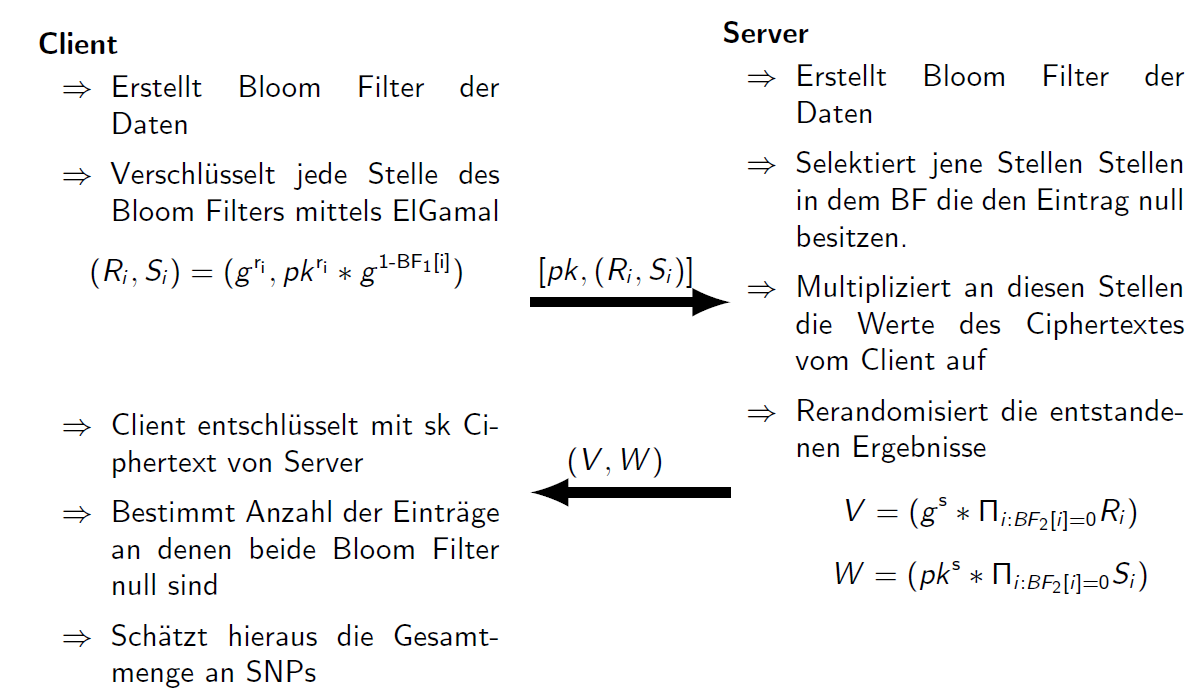
\includegraphics[width=0.7\textwidth]{Graphics/elgamal.png}
	\caption{Erstes Bild}
	\label{fig:Bild1}
\end{figure}


Dieser Algorithmus wurde zunächst im ... veröffentlicht. Es wurden Algorithmen für unterschiedliche Konstellationen postuliert. 

Der Client erstellt zu Beginn einen Boomfilter seiner Daten. Dabei wird jedes Datenelement einzeln 
Zur Verschlüsselung wählt der Client zunächst public und secret key nach elgamal.
Daraufhin wird jedes Bit des Bloomfilter Arrays einzeln verschlüsselt.
Hierzu werden die zu sendende Nachrichten so gewählt das $m = g^BF[i]$
Dies führt dazu, dass $ m $ an Stellen an welchen der Bloomfilter $ BF_Client = 0 $  dem Wert 1  entspricht und an den Stellen, an denen $ BF_Client = 1 $ dem Generator g.

\[
S\textsubscript{i} = pk^{r_{i}} \ * \ \left\{
\begin{array}{ll}
g^{0} = 1 \ bei \  BF\textsubscript{1}[i]=1\\
g^{1} = g \ bei \ BF\textsubscript{1}[i]=0\\
\end{array}
\right.
\]

Diese Nachricht wird dann nach Elgamal verschlüsselt. Der Ciphertext entspricht dann:
$$(R_i, S_i) = (g \textsuperscript{r\textsubscript{i}} , pk\textsuperscript{r\textsubscript{i}} * g\textsuperscript{1-BF\textsubscript{1}[i]})$$

Der Ciphertext wird dann zusammen mit dem public key und den Bloomfilter Parametern an den Server übermittelt.
Dieser erstellt nun seinerseits einen Bloomfilter mit den Einträgen seines Datensatzes unter Berücksichtigung der Parameter des Clients. 

Für alle Indices an welchen $BF_Server = 0$ werden die Elemente des Ciphertextes des Clients $R_i$ und $S_i$ aufmultipliziert.
Dies ist aufgrund der Homomorphie Eigenschaft von Elgamal ohne Datenverlust möglich.

Daraufhin selektiert dieser alle Indexes von Einträgen seines Bloomfilters. Indices 
Für jeden dieser Indices wird daraufhin der entsprechende Eintrag im Ciphertexts des Clients 
Aufmultiplikation  von $R_i$ bzw $S_i$ an jenen Stellen, an welchen $BF_2 = 0$ ist.

$$ V = (g^{s + r_{i_{1}} + r_{i_{2}} + \ ...\ +r_{i_{k}}})$$

\[
W =\left\{
\begin{array}{ll}
pk^{s + r_{i_{1}} + r_{i_{2}} + \ ...\ +r_{i_{l}}}*1 \ falls \ BF_{1} = 1,BF_{2} = 0 \\
pk^{s + r_{i_{1}} + r_{i_{2}} + \ ...\ +r_{i_{m}}}*g^{x} \ falls \ BF_{1} = BF_{2} = 0\\
\end{array}
\right.
\]

Die Ergebnisse werden nun mit $ g \textsuperscript{s}  $ bzw. $ pk \textsuperscript{s} $ rerandomisiert :
$$ V = (g \textsuperscript{s} * \Pi_{i:BF_{2}[i] = 0} R_{i} )$$
$$ W = (pk \textsuperscript{s} * \Pi_{i:BF_{2}[i] = 0} S_{i} )$$ \\
$ V $ und $ W $ werden nun zurück an den Client gesendet, welcher nun die Elgamal Entschlüsselung auf diese anwendet:
$$\Sigma = W * V^{-sk}$$

Da $pk$ = $g^{sk}$, ergibt sich folgende Gleichung:
	
$$\Sigma = (g^{sk * s + r_{i_{1}} + r_{i_{2}} + \ ...\ +r_{i_{k}}} \ * \ g^{-sk * s + r_{i_{1}} + r_{i_{2}} + \ ...\ +r_{i_{k}}} \ * \ g^z) $$


Nach dem Kürzen erhält man:
$$\Sigma = g^x$$

$ z $ entspricht hierbei der Anzahl an Positionen an denen sowohl der Client als auch der Server einen Nulleintag in ihren Bloomfiltern haben.

Der approximierte Betrag der im Bloomfilter gespeicherten Elemente errechnet sich dann durch:

$$ |X| = \frac{ln( \frac{z}{m})}{k* \ ln(1- \frac{1}{m})}$$



\subsection{Algorithmus 2 - Paillier}
\label{sec:Sec2.3}
 Information Security and Privacy
\begin{figure}[htbp] 
	\centering
	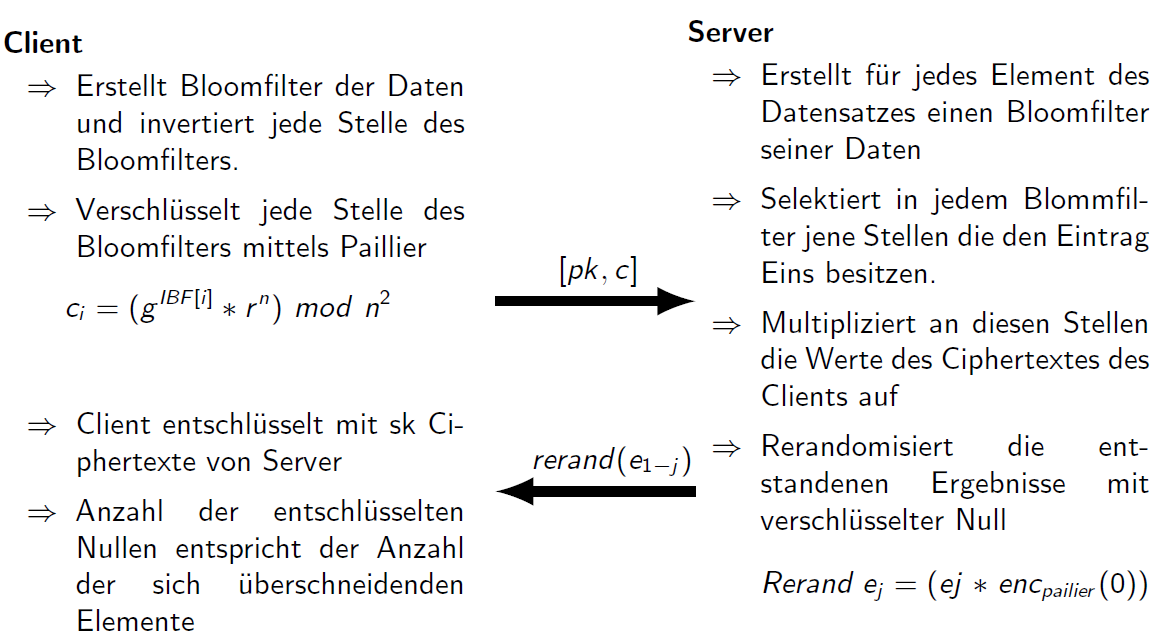
\includegraphics[width=0.7\textwidth]{Graphics/Paillier.PNG}
	\caption{Erstes Bild}
	\label{fig:Bild2}
\end{figure}

Zunächst erstellt der Client einen Bloomfilter über seine Daten.
Mittels des Pailier Kryptosystems wird wird jede Stelle des Bloomfilters einzeln verschlüsselt: 

$$c_i = (g \textsuperscript{IBF[i]}  * r_{i}\textsuperscript{n})$$

\[
C\textsubscript{i} = r_{i}^{n} \ * \ \left\{
\begin{array}{ll}
g^{0} = 1 \ bei \  BF\textsubscript{1}[i]=1\\
g^{1} = g \ bei \ BF\textsubscript{1}[i]=0\\
\end{array}
\right.
\]


pk: public key, sk: private key, g: Generator $r_i$: Zufallszahlen aus $Z_q$ 

Der Server erstellt nun für jede Stelle einen eigen Bloomfilter.
Daraufhin multipliziert er für jeden seiner Bloomfilter den Ciphertext des Clients an jenen Stellen auf, an welchen  $BF_{server[j]} = 1$.	

$$ V_{j} = (g^{ IBF_{i_{1}} + IBF_{i_{2}} + \ ...\ +IBF_{i_{k}}} \ * \ r_{i_{1}}^{n} \ * \ r_{i_{2}}^{n} \ * \ ...\ * \  r_{i_{k}}^{n})$$

\[
V_{j} = \ r_{i_{1}}^{n} \ * \ r_{i_{2}}^{n} \ * \ ...\ * \  r_{i_{k}}^{n} \ \left\{
\begin{array}{ll}
g^{1 + 1 + 1 + \ ...\ +1} \ wenn \ BF_{c} = 0,BF_{s[j]} = 1 \\
g^{0 + 0 + 0 + \ ...\ +0} \ wenn \ BF_{c} = BF_{s[j]} = 1\\
\end{array}
\right.
\]




$$\Sigma = W * V^{-sk}$$

V, W aus vorherigem Schritt einsetzen und für $pk$ = $g^{sk}$ 

\vskip 0.1cm 

$$\Sigma = (g^{sk * s + r_{i_{1}} + r_{i_{2}} + \ ...\ +r_{i_{k}}} \ * \ g^{-sk * s + r_{i_{1}} + r_{i_{2}} + \ ...\ +r_{i_{k}}} \ * \ g^x) $$
$$\Sigma = g^x$$




The number of hash functions has distinct less influence 







